%  !TeX  root  =  user_guide.tex

\section{Oracle GeoRaster Plugin}

% when the revision of a section has been finalized, 
% comment out the following line:
% \updatedisclaimer

In Oracle databases, raster data can be stored in SDO\_GEORASTER objects available with the 
Oracle Spatial extension. In QGIS, the \toolbtntwo{oracle_raster}{Oracle GeoRaster Plugin} 
is supported by GDAL, and depends on Oracle's Database product being installed and working 
on your machine. While Oracle is proprietary software, they provide their software free for 
development and testing purposes. Here is one simple example of how to load raster images 
to GeoRaster:

\begin{verbatim} 
$ gdal_translate -of georaster input_file.tif geor:scott/tiger@orcl
\end{verbatim}

This will load the raster into the default GDAL\_IMPORT table, as a column named RASTER.

\subsection{Managing connections}

Firstly, the Oracle GeoRaster Plugin must be enabled using the Plugin Manager (see Section 
\ref{sec:load_core_plugin}). The first time you load a GeoRaster in QGIS, you must create a 
connection to the Oracle database that contains the data. To do this, begin by clicking on 
the \toolbtntwo{oracle_raster}{Select GeoRaster} toolbar button, it will open the Select Oracle 
Spatial GeoRaster dialog window. Click on \button{New} to open the dialog window, and specify 
the connection parameters (See Figure \ref{fig:oracle_create}):

\begin{itemize}[label=--]
\item \textbf{Name}: Enter a name for the database connection.
\item \textbf{Database instance}: Enter the name of the database that you will connect to.
\item \textbf{Username}: Specify your own username that you will use to access the database.
\item \textbf{Password}: The password associated with your username that is required to access the database.
\end{itemize}

\begin{figure}[ht]
   \centering
   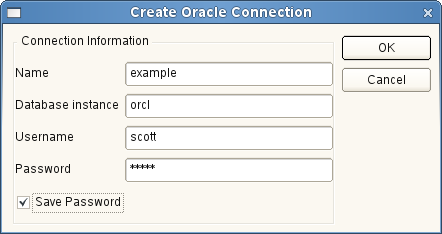
\includegraphics[clip=true, width=9cm]{oracle_create_dialog}   
   \caption{Create Oracle connection dialog \nixcaption}\label{fig:oracle_create}
\end{figure}

Now, back on the main Oracle Spatial GeoRaster dialog window (See Figure \ref{fig:oracle_select}), use the 
drop-down list to choose one connection, and use the \button{Connect} button to establish a connection. You 
may also \button{Edit} the connection by opening the previous dialog and making changes to the connection 
information, or use the \button{Delete} button to remove the connection from the drop-down list.

\subsection{Selecting a GeoRaster}

Once a connection has been established, the sub-datasets window will show the names of all the tables that 
contains GeoRaster columns in that database in the format of a GDAL subdataset name.

Click on one of the listed subdatasets and then click on \button{Select} to choose the table name. Now another 
list of subdatasets will show with the names of GeoRaster columns on that table. This is usually a short list, 
since most users will not have more than one or two GeoRaster columns on the same table.

Click on one of the listed subdatasets and then click on \button{Select} to choose one of the the table/column 
combination. The dialog will now show all the rows that contains GeoRaster objects. Note that the subdataset 
list will now show the Raster Data Table and Raster Id's pairs.

At anytime the Selection entry can be edited in order to go directly to a known GeoRaster or to go back to the 
beginning and select another table name.

\begin{figure}[ht]
   \centering
   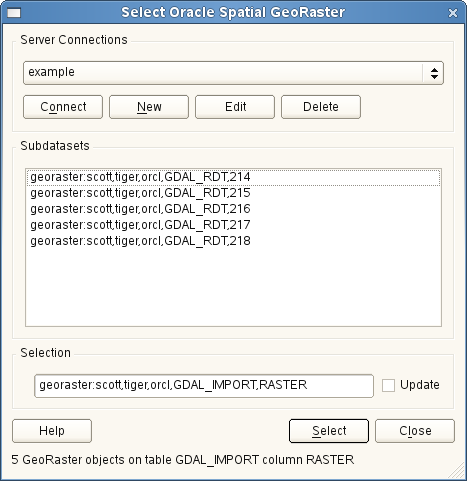
\includegraphics[clip=true, width=9cm]{oracle_select_dialog}   
   \caption{Select Oracle GeoRaster dialog \nixcaption}\label{fig:oracle_select}
\end{figure}

The Selection data entry can also be used to enter a Where clause at the end of the  identification string, e.g., 
``geor:scott/tiger@orcl,gdal\_import,raster,geoid=''. See \url{http://www.gdal.org/frmt_georaster.html} for more information.

\subsection{Displaying GeoRaster}

Finally, by selecting a GeoRaster from the list of Raster Data Table and Raster Id's, the raster image will be 
loaded into QGIS.

The Select Oracle Spatial GeoRaster dialog window can be closed now and next time it opens it will keep the same 
connection, and will show the same previous list of subdataset making it very easy to open up another image 
from the same context.

\textbf{Note:} GeoRasters that contains pyramids will display much faster but the pyramids need to be generated 
outside of QGIS using Oracle PL/SQL or gdaladdo.

The following is example using gdaladdo:

\begin{verbatim}
gdaladdo georaster:scott/tiger@orcl,georaster\_table,georaster,georid=6 -r 
nearest 2 4 6 8 16 32
\end{verbatim}

This is an example using PL/SQL: 
cd ..
\begin{verbatim}
$ sqlplus scott/tiger
SQL> DECLARE
    gr sdo_georaster;
BEGIN
    SELECT image INTO gr FROM cities WHERE id = 1 FOR UPDATE;
    sdo_geor.generatePyramid(gr, 'rLevel=5, resampling=NN');
    UPDATE cities SET image = gr WHERE id = 1;
    COMMIT;
END;
/
\end{verbatim}

\FloatBarrier
